\documentclass[xcolor=pdftex,dvipsnames,table,mathserif]{beamer}
%\usepackage{subfigure}
\usepackage{amsbsy}
\usepackage{tikz}
\usetikzlibrary{arrows}
\usepackage{amsmath,graphicx,dsfont,color}
\usepackage{amsfonts}
\usepackage{amssymb}
\usepackage{array}

\usepackage{subfig}

% makes the subfig package work
\makeatletter
\let\@@magyar@captionfix\relax
\makeatother

% subfigure counter resets every frame
\makeatletter
\@addtoreset{subfigure}{framenumber}
\makeatother

% First author and year
\bibliographystyle{apalike}

% This sets the list items of the bibliography to the same symbol used for citation.
\setbeamertemplate{bibliography item}{\insertbiblabel}

% This avoids extralines for different entries
\setbeamertemplate{bibliography entry title}{}
\setbeamertemplate{bibliography entry location}{}
\setbeamertemplate{bibliography entry note}{}

\DeclareMathOperator*{\argmin}{arg\,min}
\DeclareMathOperator*{\argmax}{arg\,max}
%Definitiona

\newcommand{\x}{\mathbf{x}}
\newcommand{\X}{\mathbf{X}}
\newcommand{\W}{\mathbf{W}} %Weight
\newcommand{\bais}{\mathbf{b}}%Bais
\newcommand{\act}{\texttt{g}}%Activation
\newcommand{\loss}{L}
\newcommand{\pdata}{\hat{p}_{\texttt{data}}}
\newcommand{\nsize}{N}
\newcommand{\nfeatures}{P}
\newcommand{\param}{\boldsymbol{\theta}}
\newcommand{\featmap}{\boldsymbol{\phi}}
\newcommand{\EV}{\mathbb{E}}







\usepackage{physics}

\graphicspath{{../graphics/}}

\AtBeginSection[]{
  \begin{frame}{Contents}
    \tableofcontents[currentsection, hideothersubsections]
  \end{frame}
}

\AtBeginSubsection[]{
  \begin{frame}{Contents}
    \tableofcontents[currentsection, subsectionstyle=show/shaded/hide]
  \end{frame}
}

\setbeamertemplate{footline}[frame number]{}
\setbeamertemplate{navigation symbols}{}
\setbeamertemplate{section in toc}[square]
\setbeamertemplate{items}[square]

%% For image credits on image bottom right
\usepackage[absolute,overlay]{textpos}
\setbeamercolor{framesource}{fg=gray}
\setbeamerfont{framesource}{size=\tiny}
\newcommand{\source}[1]{\begin{textblock*}{4cm}(8.7cm,8.6cm)
    \begin{beamercolorbox}[ht=0.5cm,right]{framesource}
      \usebeamerfont{framesource}\usebeamercolor[fg]{framesource} Credits: {#1}
    \end{beamercolorbox}
\end{textblock*}}

\title{Unsupervised anomalous image detection}
\author{E. Decencière}
\date{MINES ParisTech\\
  PSL Research University\\
  Center for Mathematical Morphology
}
\titlegraphic{
\includegraphics[height=1.7cm]{../graphics/logoemp}}

\useinnertheme{rounded}
\usecolortheme{rose}

%%%%%%%%%%%%%%%%%%%%%%%%%%%%%%%%%%%%%%%%%%%%%%%%%%%%%%%
%%%%%%%%%%%%%%%%%%%%%%%%%%%%%%%%%%%%%%%%%%%%%%%%%%%%%%%

\begin{document}

\frame{\titlepage}

\frame{
  \frametitle{Contents}
  \tableofcontents[hidesubsections]
}

%%%%%%%%%%%%%%%%%%%%%%%%%%%%%%%%%%%%%%%%%%%%%%%%%%
%%%%%%%%%%%%%%%%%%%%%%%%%%%%%%%%%%%%%%%%%%%%%%%%%%
\section{Introduction}

%%%%%%%%%%%%%%%%%%%%%%%%%%%%%%%%%%%%
\begin{frame}{Definition in layman terms}


  \begin{block}{Anomaly detection}
  Let us consider a given kind of objects (for example, images). Among these objects, some  are defined as being \alert{normal}. The aim of the detection task is to decide, for a given object, if it is normal, or not.

  The definition of normal objects is given through a set of examples.
  \end{block}

  \begin{itemize}
  \item   We will focus on images, but the problem is very general.
  \item We will suppose that we only have examples of normal objects, i.e. that we are in a \alert{unsupervised} context. We assume that examples of anomalies are not representative enough.
  \end{itemize}



\end{frame}

%%%%%%%%%%%%%%%%%%%%%%%%%%%%%%%%%%%%
\begin{frame}{Example - set of normal images}

\begin{figure}[ht]
  \centering
  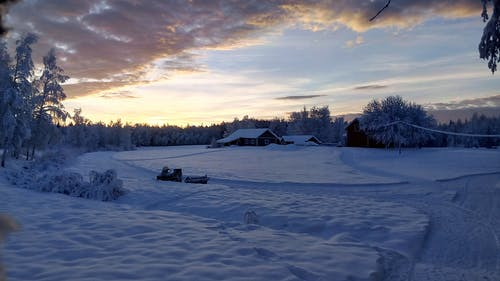
\includegraphics[width=0.3\textwidth]{snow1-pexels-photo-290548.jpg}
  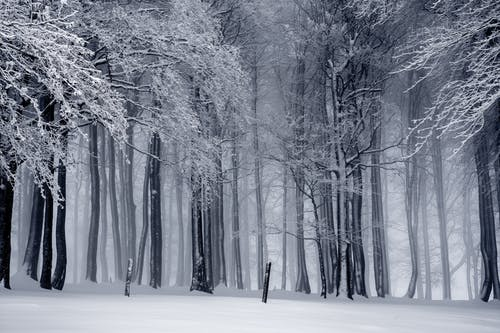
\includegraphics[width=0.3\textwidth]{snow2-pexels-photo-235621.jpg}
  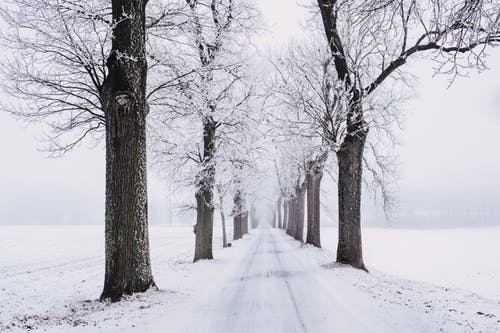
\includegraphics[width=0.3\textwidth]{snow3-pexels-photo-839462.jpeg}
  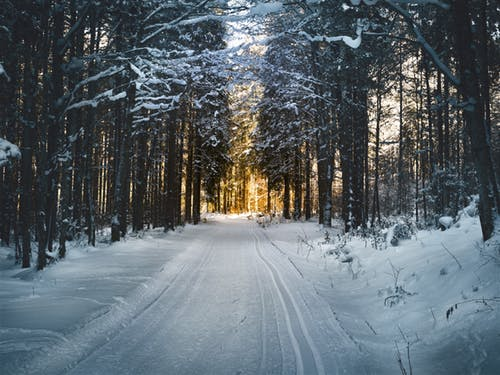
\includegraphics[width=0.3\textwidth]{snow4-pexels-photo-688660.jpeg}
  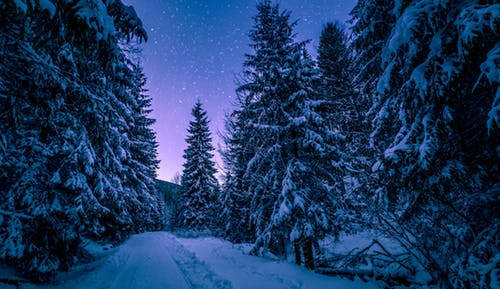
\includegraphics[width=0.3\textwidth]{snow5-pexels-photo-773594.jpeg}
  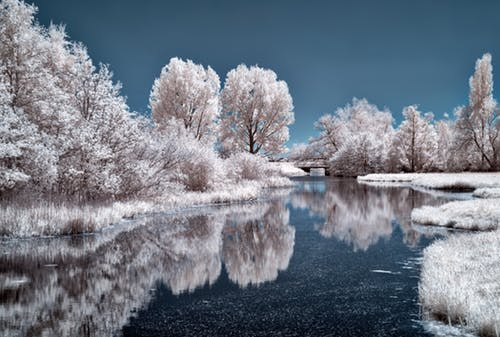
\includegraphics[width=0.3\textwidth]{snow6-pexels-photo-1559117.jpeg}
  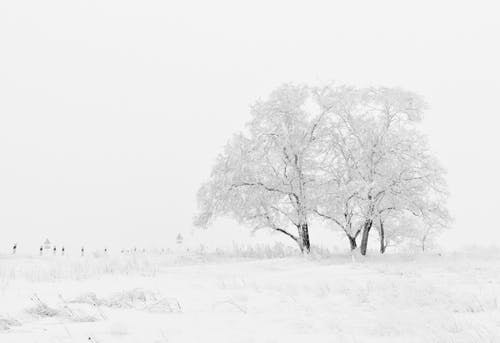
\includegraphics[width=0.3\textwidth]{snow7-pexels-photo-66284.jpeg}
  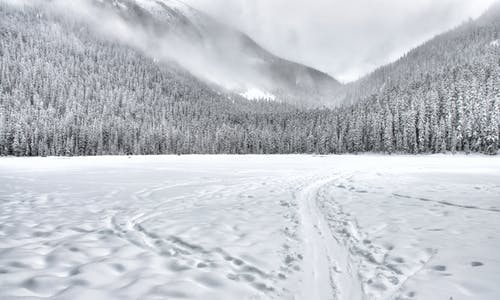
\includegraphics[width=0.3\textwidth]{snow8-pexels-photo-1571442.jpeg}
  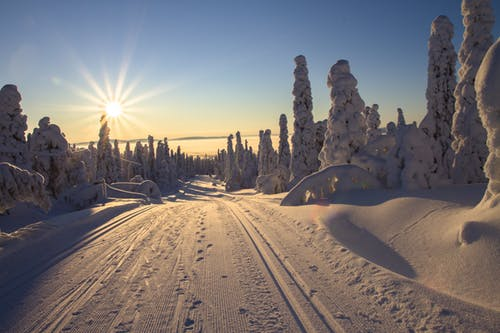
\includegraphics[width=0.3\textwidth]{snow9-pexels-photo-416728.jpeg}\
  \source{http://pexels.com}
\end{figure}

\end{frame}

%%%%%%%%%%%%%%%%%%%%%%%%%%%%%%%%%%%%
\begin{frame}{Example - which images are normal?}

\begin{figure}[ht]
  \centering
  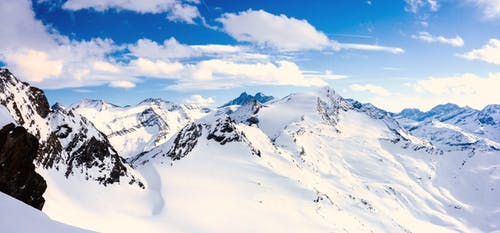
\includegraphics[width=0.3\textwidth]{test1-pexels-photo-414459.jpeg}
  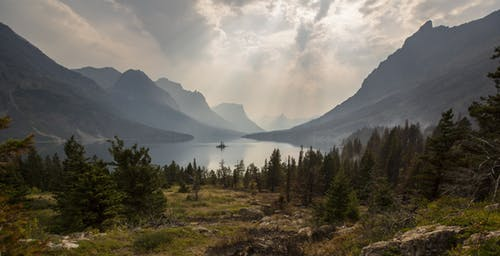
\includegraphics[width=0.3\textwidth]{test2-pexels-photo-414171.jpeg}
  \source{http://pexels.com}
\end{figure}

\end{frame}


%%%%%%%%%%%%%%%%%%%%%%%%%%%%%%%%%%%%
\begin{frame}{Application: security}

\begin{itemize}
\item Suspicious object or unusual behaviour in a scene
\end{itemize}

\begin{figure}[ht]
  \centering
  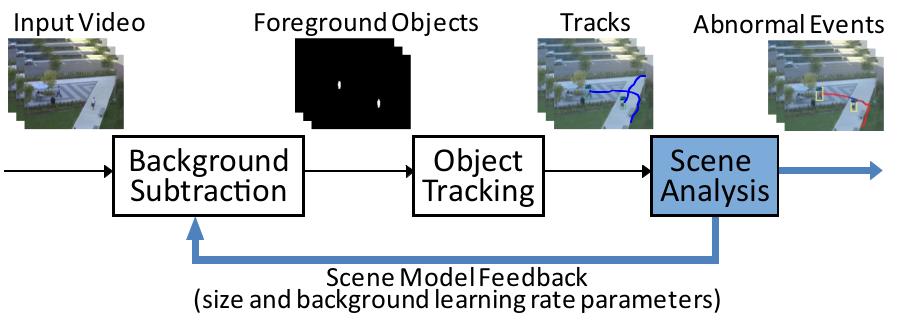
\includegraphics[width=0.8\textwidth]{motion_patterns_anom_det}
  \caption{\cite{basharat_learning_2008}}
\end{figure}


\end{frame}

%%%%%%%%%%%%%%%%%%%%%%%%%%%%%%%%%%%%
\begin{frame}{Application: industrial control}

  \begin{itemize}
  \item Fault detection
  \item Structural defect detection
   \end{itemize}

\begin{figure}[ht]
  \centering
  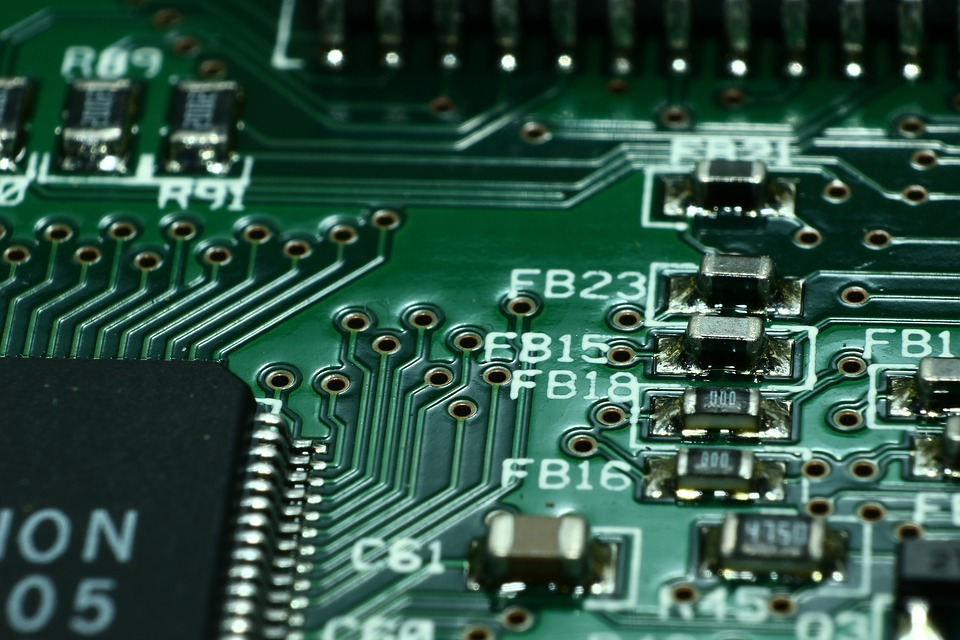
\includegraphics[width=0.5\textwidth]{printed-circuit-board-1539113_960_720.jpg}
  \source{http://www.pixabay.com}
\end{figure}


\end{frame}

%%%%%%%%%%%%%%%%%%%%%%%%%%%%%%%%%%%%
\begin{frame}{Medicine}

  \begin{itemize}
  \item Detection of suspicious conditions
  \item Non specific screening
  \end{itemize}

\begin{figure}[ht]
  \centering
  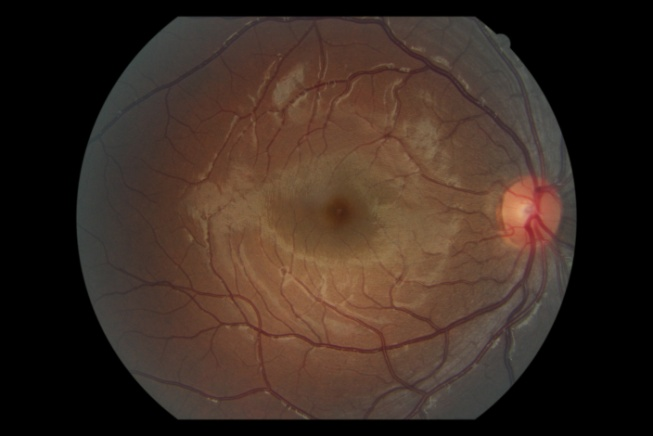
\includegraphics[width=0.5\textwidth]{fundus1}
  \caption{Retinal image used for pathology screening}
  \source{OPHDIAT database}
\end{figure}


\end{frame}


%%%%%%%%%%%%%%%%%%%%%%%%%%%%%%%%%%%%
\begin{frame}{Science}

  \begin{itemize}
  \item In some fields so many images are generated that it is becoming impossible to look at all of them
  \item Example: Euclid telescope (European Space Agency and Euclid consortium)
  \end{itemize}

  \begin{figure}[ht]
    \centering
    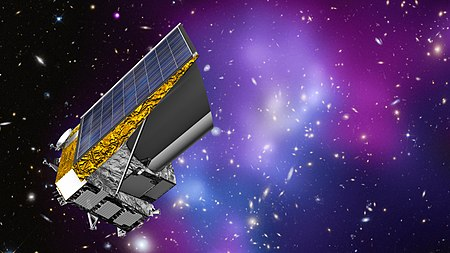
\includegraphics[width=0.5\textwidth]{450px-Euclid_ESA376594}
    \source{https://sci.esa.int/web/euclid/}
  \end{figure}


\end{frame}


%%%%%%%%%%%%%%%%%%%%%%%%%%%%%%%%%%%%
\begin{frame}{Euclid project}

\begin{itemize}
\item A new space telescope, to be launched in 2022
\item Its objective is improving our understanding of the acceleration of the universe expansion
\item To do so, the shapes of galaxies at different distances from the earth will be measured
\item An estimated $10^{10}$ extra galactic objects will be acquired by the telescope
\item Data will be automatically analyzed, without visual inspection
\end{itemize}

  \begin{figure}[ht]
    \centering
    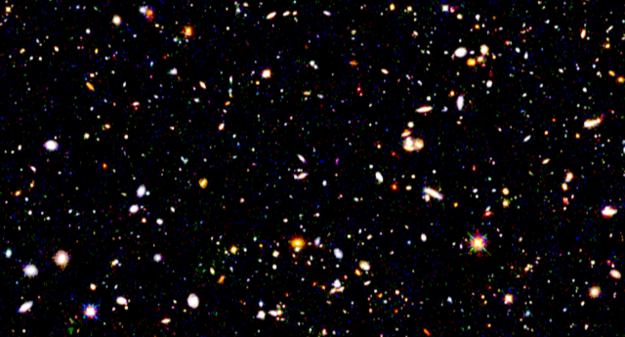
\includegraphics[width=0.5\textwidth]{ESA_Euclid_EDFF_Candels_v1_zoom_625}
    \source{https://sci.esa.int}
  \end{figure}

\end{frame}

%%%%%%%%%%%%%%%%%%%%%%%%%%%%%%%%%%%%
\begin{frame}{Vocabulary}

  \begin{itemize}
  \item Anomaly
  \item Novelty
  \item Outlier
  \end{itemize}

  In machine learning: one-class classification.
\end{frame}


%%%%%%%%%%%%%%%%%%%%%%%
%%%%%%%%%%%%%%%%%%%%%%%
\section{Mathematical modelling}

%%%%%%%%%%%%%%%%%%%%%%%%%%%%%%%%%%%%
\begin{frame}{Basic principles}

  \begin{itemize}
  \item   Let $E$ be a set (the whole set of objects), $\mathcal{N}$ the subset of $E$ (constituted by all normal objects) and $X$ a subset of $N$ (the set of examples that are considered to be \emph{normal}).
  \item The question we would like to answer is:

    \begin{block}{}
      \centering
    Is a given $x$ in $E$ normal?
    \end{block}

    \item What should we add to our definition of $E$ and $X$ for this question to be meaningful?
  \end{itemize}

  Some possibilities:
  \begin{itemize}
  \item Metric space
  \item Probability space
  \end{itemize}

\end{frame}


%%%%%%%%%%%%%%%%%%%%%%%%%%%%%%%%%%%%
\begin{frame}{Metric space}

  $E$ is equipped with a distance $d$. We then can answer the question if there is a distance value $d_0$ such that:
  \[
  x \in \mathcal{N} \iff d(x, X) \leq d_0
  \]

  Of course, the essential point will be then how to choose the distance function $d$.

\end{frame}


%%%%%%%%%%%%%%%%%%%%%%%%%%%%%%%%%%%%
\begin{frame}{Probabilistic approach}

  In order to probabilise $E$ we need a $sigma$-algebra $\mathcal{A}$ (the events set) and a probability measure $P$.



\end{frame}




%%%%%%%%%%%%%%%%%%%%%%%%%%%%%%%%%%%%%%%%%%%%%%%%%%
\section*{References}

%%%%%%%%%%%%%%%%%%%%%%%%%%%%%%%%%%%%%%%%%%%%%%%%%%

\frame[allowframebreaks]{

  \scriptsize

  \frametitle{References}

  %\bibliographystyle{amsalpha}
  %\bibliographystyle{apalike}

  \bibliography{../../edf.bib}

  \normalsize

}




\end{document}
